%% Generated by tools/md2tex.js from paper/p2.md. Do not edit by hand: edit
%% p2.md, then run  node tools/md2tex.js p2  and recompile.
\documentclass[11pt]{article}
\usepackage[T1]{fontenc}
\usepackage{lmodern}
\usepackage[utf8]{inputenc}
\usepackage[margin=1in]{geometry}
\usepackage{booktabs,graphicx,amsmath,amssymb}
\graphicspath{{../}}
\usepackage{tabularx}
\usepackage[numbers,sort&compress]{natbib}
\usepackage{threeparttablex}
\usepackage[british]{babel}
\usepackage[hidelinks]{hyperref}
\setlength{\bibsep}{4pt}
% [S#] is a provenance tag. Each one resolves to a row of the appendix table in
% p2.md, which paper/tex_audit-p2.md re-checks file by file. It is rendered as a
% small superscript rather than dropped, so an unresolved tag stays visible.
\newcommand{\prov}[1]{\textsuperscript{\,#1}}
\widowpenalty=10000
\clubpenalty=10000
\tolerance=2000
\emergencystretch=2em
\title{P2 --- Certified screening of the VV10 nonlocal-correlation double sum: what the bound buys, and what it costs}
\author{Angran Xia\thanks{Corresponding author; e-mail in the byline.} \\ \small \textit{School of Chemistry \& Chemical Engineering, Shaanxi Normal University, Xi'an 710119, Shaanxi, China} \\ \small \texttt{haangyeon@snnu.edu.cn} \and Changwei Wang \\ \small \textit{School of Chemistry \& Chemical Engineering, Shaanxi Normal University, Xi'an 710119, Shaanxi, China}}
\date{Draft --- 29 September 2026\\ \small \textit{ORCIDs PENDING, author-supplied}}
\begin{document}
\maketitle
\textbf{Status, 2026-10-02 --- merged, and not to be submitted separately while P1 is under review.} The measurements in sections 3, 6 and 7 are carried by \texttt{paper/main.md} \S{}3.6 in the form that paper's argument needs: the two wall-clock windows (1.08-10.28x and 1.37-13.29x over 33 timed pairs, none faster), the 197.96 Ha certificate against a -8.34e-4 Ha quantity, and the 84.4-95.4\% of far-field pairs evaluated at the tolerance that still meets 1e-6 kcal/mol. Two sections are \emph{not} in that condensation and are the reason this file is kept rather than deleted: section 4's survey of which geometric criterion can screen at all, and section 5's account of where the bound's tightness actually comes from. If a second, algorithm-shaped submission is ever wanted, those two are its spine - but submitting this text alongside \texttt{main.md} would put overlapping prose in front of the same reviewers, so the choice is made explicitly here rather than left to whoever finds the file.

\textbf{Authors.} Angran Xia (corresponding; \texttt{haangyeon@snnu.edu.cn}) and Changwei Wang --- School of Chemistry \& Chemical Engineering, Shaanxi Normal University, Chang'an Campus, Xi'an 710119, Shaanxi, China. Names, institution and the corresponding e-mail were supplied by the author on 2026-09-30; the college's English wording is taken from the college's own English site and the campus postal code from the university's contact page. The authors' Chinese names live in \texttt{paper/software.md}'s front matter and \texttt{CITATION.cff}, not here: the P1 pipeline typesets with pdflatex, which has no CJK font, and the same rule is applied to all three manuscripts. ORCIDs and the second author's e-mail remain PENDING (author-supplied).

\section{Abstract}

The VV10 nonlocal-correlation term of omegaB97X-V is evaluated as a double sum over real-space integration points, so its cost is quadratic in the number of points. We implemented a \emph{certified} screening scheme for it: every pair of grid-point blocks is either evaluated exactly or replaced by an upper bound proved to dominate its contribution, the bounds accumulate into one pre-declared error, and the point-pair structure is kept intact so the result can still be attributed fragment by fragment. We then measured the scheme against the dense sum under a recorded contention gate, and report that it does not pay. At the accuracy a fragment-pair decomposition needs (1e-6 kcal/mol per pair term) the bound is so loose that 84.4-95.4\% of the far-field point pairs must still be evaluated; of the 33 screened-versus-exact pairs sampled in two independent timing windows on one machine, none was faster than the dense sum, and the largest slowdown measured is 13.29x. Three measurements explain the outcome and are the substance of this paper. At atom-block granularity the \emph{smallest} block-pair bound in a real dimer exceeds the whole quantity it is supposed to judge by a factor of 2.4e5. Every root box separation in the dimers studied is exactly 0.0000 A, so the near field is 100\% of the cross point pairs and a geometric accept/reject rule has a 0.0\% saving ceiling. Tightening the bound by splitting each block into a dense core and a sparse tail raises the fraction of droppable point pairs only from 12.349\% to 13.650\%. One criterion that looks obviously monotone under refinement - a mass-weighted ball - loses the property on 18\% of refinements, found only by counting. We state the four conditions a certified scheme would have to meet before it could win, note that none holds for weakly bound dimers, and keep the screening off by default.

\section{1. What we built, what it measured, and what was already known}

\emph{Screening} in this paper is an algorithmic sparsity truncation with a proof attached: a block pair is skipped only when an upper bound on its contribution, computed before the skip, dominates everything that would have been lost. It is not the Lindhard/dielectric screening that the vdW-DF literature also calls "screening", and we avoid that reading by never calling the kernel screened --- only the sum is.

The VV10 nonlocal-correlation energy of $\omega$B97X-V is evaluated as a bilinear form over a real-space integration grid, and the cost is quadratic in the number of retained grid points. We built a scheme that keeps the exact value for the block pairs it evaluates and carries a \textbf{certified} upper bound for the ones it drops, accumulated into a single pre-declared \texttt{cert\_err}, while preserving the grid-point-pair structure that a fragment-pair energy decomposition needs (P1's quantity). Then we measured it, and the measurement is the paper:

- at the accuracy the decomposition requires (1e-6 kcal/mol on a fragment-pair term), the   screened path still evaluates \textbf{84.4-95.4\%} of the far-field point pairs; - with no other runnable user task at the sampling instant (external R-state count 0;   \texttt{load1} is recorded, 0.99-4.24, but the core count is not, so this is a contention gate   and \textbf{not} a claim that the box was idle), across 24 timed runs in the archived window and   20 in a second independent one --- 33 screened/exact pairs in total --- the screened path is   \textbf{1.08-10.28$\times$ slower} in the first window and \textbf{1.37-13.29$\times$} in the second, never faster;   at the tightest tolerance tested ($\tau$ = 1e-12 Ha), counting every row at that tolerance, the penalty is   \textbf{1.95-10.28$\times$} and \textbf{2.63-13.29$\times$} (\textbf{1.95-10.85$\times$} over the eight rows that meet the target),   and even there 3 of the 11 timed rows still miss the 1e-6 kcal/mol target: 1.8e-6 in the   12-atom level-0 row of each window, 1.5e-6 in the 9-atom level-1 row of the archived one   (\S{}6); - the reason is visible in the bound itself: at atom-block granularity the \emph{smallest}   block-pair bound in a real water dimer exceeds the entire quantity it is meant to judge   by a factor of \textbf{2.4e5}, and the near field accounts for \textbf{100\%} of the cross   point-pairs --- every root box separation is exactly 0.0000 \AA{} (\S{}3, \S{}5).

\textbf{What is not new.} Making this double sum cheaper is a live target. VV10 itself was introduced as a closed-form kernel replacing the adiabatic-connection integrand \citep{vydrov2009vv10}, with a separable/efficient form soon after \citep{vydrov2010simple}; \citep{sabatini2013efficient}, and real-space grid implementations with parallel post-processing exist \citep{lazic2010junolo}. The nearest current work is Laikov's preprint "Nonlocal van der Waals density functional made faster" \citep{laikov2026faster} (v2, 2026-01-19), which \emph{approximates the six-dimensional integrand by products of three-dimensional density-like distributions and potential-like functions of the interelectronic distance}, explicitly to open it to fast-multipole evaluation, with a Gaussian-fitted analytic variant on top; the claimed accuracy is empirical --- its own noble-gas-dimer table gives a well-depth deviation of 103.6 $\mu$Eh for XeXe, and its text assesses the tuned variant as "below 18 \%" for bond energies (mostly below 1.2 \% for bond lengths) --- no tolerance parameter and no bound are given, and the pairwise accumulation structure is not what the method returns. Read end to end, it is a \emph{kernel replacement}: an empirically tuned separable rational expansion standing in for VV10's $\Phi$, which is the right move when only the total is wanted. We screen the original sum, which is the only move available when the answer must be a pair-by-pair attribution --- and we measure what preserving it costs. Efficient real-space evaluation of a nonlocal term is also established for periodic codes \citep{nabok2011noloco} and in the vdW-DF grid implementations cited above. Hierarchical box/MAC machinery with provable geometric error bounds is classical for Coulomb integrals and exact exchange \citep{schwegler1998multipole}; \citep{dehnen2002hierarchical}. The abbreviation "JCP" is deliberately spelled out in both halves of that pair: the two papers sit in different journals whose initials collide, and a reader who goes looking in one finds nothing. The closest \emph{mechanism} neighbour is not a nonlocal-term paper at all: the "Linear Scaling Hierarchical Integration Scheme for the Exchange-Correlation Term" of Burow \& Sierka \citep{burow2011hierarchical} octrees the grid and screens negligible contributions adaptively --- for a \emph{single} integral over a semi-local functional, with no rigorous bound and no pair attribution. The "have a proof" half of our conjunction likewise has ancestry outside this object: rigorous multipole upper bounds for electron-repulsion integrals \citep{lambrecht2005estimates}; \citep{lambrecht2005screening}; \citep{doser2008tighter} and a rigorous relative-error criterion for tree/FMM summation of Newton potentials \citep{engblom2011wellseparated}. The object is what is unclaimed: $\iint$ $\rho$ $\Phi$ $\rho$ with VV10's $\Phi$, screened by a proven bound, with the pair ledger intact.

\textbf{Publishing a refutation is not new either}, and we say so deliberately: the "which fast scheme is actually faster at molecular sizes" comparison is a mature genre in electrostatics and N-body work \citep{luty1994pppmesh}; \citep{petersen1995pmesh}; \citep{deserno1998meshup}; \citep{gumerov2008fmmgpu}; \citep{kohnke2020gmxfmm}, where the crossover size is known to depend on the kernel and the constants rather than on the asymptotic exponent. Our result is that same shape of measurement for a different bilinear form, and we cite these as methodological neighbours rather than as prior art on VV10.

\textbf{Scope, and how confident the novelty statement is.} We claim: (i) a certified per-block- pair upper bound for the VV10 real-space double sum, (ii) that it is implemented without destroying the pair attribution, and (iii) the quantitative cost measurement of (i)+(ii) against the dense kernel. We do not claim the first hierarchical or fast-multipole treatment of a nonlocal correlation term. The literature screen behind those sentences is \texttt{RESEARCH-20260930-p2-novelty.md}: 44 Web-of-Science Core Collection search strings executed through the site's own record endpoint with six known-item calibrations passing, plus Crossref, OpenAlex and arXiv, every string and hit count logged. Its limits are stated in the same file and are not small: three of the five citation-hub sweeps attempted (Sabatini, with 738 records, Gulans with 167, JuNoLo with 47) were cut off by HTTP 429 at the first page and returned nothing, while the two that completed were the Laikov hub (0 citations, so no indexed follow-up exists yet) and the Román-Pérez \& Soler hub (1,596 fetched against a server count of 1,590, reconciliation passed, one title hit and it is a review); a sixth hub we named was never swept at all. Semantic Scholar was never retrieved, Scopus was not searched, and the body text of the implementation papers - where an empirical cutoff would be documented - was read only where an open copy existed. Four method names carried in our own earlier notes could not be located in any of five indexes and are therefore not named anywhere above. The novelty statement should be read as "not found in that coverage", not "does not exist"; the likeliest collision is a journal version of Laikov's preprint adding an error analysis, and this section must be re-run before submission.

\section{2. Setting}

The nonlocal-correlation term of a VV10-type functional is a double sum over numerical integration points,

    E\_NL = 1/2 $\Sigma$\_i $\Sigma$\_j w\_i $\rho$\_i w\_j $\rho$\_j $\Phi$(g\_ij, g'\_ij),      $\Phi$ = $-$3 / (2 g g' (g + g'))

with \texttt{g = w0(r\_j) R\_ij$^{2}$ + $\kappa$(r\_i)} under same-centre pairing, \texttt{w0 = sqrt(C|$\nabla$$\rho$|$^{4}$/$\rho$$^{4}$ + (4$\pi$/3)$\rho$)} ($\sigma$ = |$\nabla$$\rho$|$^{2}$, so $\sigma$$^{2}$ enters) and \texttt{$\kappa$ = b(3$\pi$/2)($\rho$/9$\pi$)\textasciicircum{}{1/6}} (b = 6.0, C = 0.01) [\texttt{nlcsplit/nlc.py:31-43}; the pairing convention and its cost are established in P1 \S{}2.1]. The reported quantity adds the local part \texttt{E\_loc = $\beta$$\int$$\rho$}, \texttt{$\beta$ = (1/32)(3/b$^{2}$)\textasciicircum{}{3/4}} [\texttt{nlcsplit/nlc.py:112}].

Two properties of this sum decide everything below.

\textbf{(i) There is no sign cancellation inside a block.} $\rho$ $\geq$ 0, the integration weights enter through \texttt{w$\rho$}, and $\Phi$ < 0 everywhere, so a block sum is bounded by the sum of absolute values without loss [\texttt{nlcsplit/fastpair.py:17-18}]. Using \texttt{m\_P = $\Sigma$\_{i$\in$P}|w\_i $\rho$\_i|} is therefore not a looseness introduced for convenience --- it is the only quantity the integrands control.

\textbf{(ii) The attribution structure is the product, not the sum.} We keep \texttt{pairs[(A,B)]} for atom (or fragment) blocks P, Q, so \texttt{E\_pair = $\Sigma$\_a v(a,a) + 2 $\Sigma$\_{a<b} v(a,b)} and the factor of two is applied exactly once, at block level [\texttt{nlcsplit/tests/test\_fastpair.py::test\_x2\_not\_applied\_twice}; the half-block convention of \texttt{nlc.pair\_energy} is documented at \texttt{nlcsplit/step\_d\_floor.py:18}]. A point-value kernel evaluation returns \texttt{dE\_NLC} and nothing else; the pair structure is what a screening scheme has to preserve to be usable for the attribution question P1 asks.

\textbf{Two independent truncations, reported separately.} The density floor \texttt{RHO\_FLOOR = 1e-12} [\texttt{nlcsplit/nlc.py:27}] already discards points before any geometry is consulted: on the water dimer at grid level 1 it keeps 17,227 of 19,936 points [\texttt{evidence/coretail/20260929T130257Z\_coretail\_bound.out}, line 3; the same two counts appear as \texttt{n\_grid} and \texttt{n\_kept} in \texttt{evidence/fastpair\_ab/fastpair\_ab\_compare.json}]. What the floor alone costs is what \texttt{nlcsplit/step\_d\_floor.py} measures. Screening is a second, orthogonal truncation. Conflating them would make the certified error meaningless, so every number below is reported with the floor held fixed and the screening budget accounted separately.

\section{3. A certified block-pair bound}

For a block pair (P, Q) with axis-aligned bounding boxes, let \texttt{D} be the box separation (\texttt{D = 0} when the boxes overlap) and

    a\_P = w0\_min(P)$\cdot$D$^{2}$ + $\kappa$\_min(P),      bound(P,Q) = 0.75$\cdot$m\_P$\cdot$m\_Q / (a\_P a\_Q (a\_P + a\_Q)).

Then \texttt{|$\Sigma$\_{i$\in$P} $\Sigma$\_{j$\in$Q} w\_i $\rho$\_i w\_j $\rho$\_j $\Phi$\_ij| $\leq$ bound(P,Q)}, and for a same-level block pair the $\times$2 convention gives \texttt{mult = 2.0}. It is applied once, at the \texttt{\_mac} call site inside \texttt{nlcsplit/fastpair.py::screened\_decomposition}; the accept/reject recursion itself is \texttt{nlcsplit/fastpair.py::\_mac}, and the bound function is \texttt{nlcsplit/fastpair.py::node\_bound}.

The bound is not tight by construction --- it is tight \emph{enough to be the thing we measure}. On real water-dimer fields the worst ratio over 390 sampled leaf pairs is \texttt{bound/|actual| = 1.181e+07} for the whole-block bound [\texttt{evidence/coretail/20260929T130257Z\_coretail\_bound.out}, Q2c, lines 134 and 147] --- a factor above ten to the seventh power, which is the honest starting point for \S{}4--\S{}6.

\textbf{What a global minimum does not buy.} A bound built from one global \texttt{w0\_min}/\texttt{$\kappa$\_min} is useless rather than merely loose, and how useless it is gets fixed by the density floor, not by any one measurement. Every retained point has \texttt{rho > 1e-12} [\texttt{nlcsplit/nlc.py:27}], and at that floor with \texttt{$\sigma$ = 0} the \S{}2 formulas give \texttt{$\kappa$\_min = 6.0$\cdot$(3$\pi$/2)$\cdot$(1e-12/9$\pi$)\textasciicircum{}{1/6} = 0.161992} and \texttt{w0\_min = sqrt((4$\pi$/3)$\cdot$1e-12) = 2.046653e-06}, evaluated by \texttt{nlc.vv10\_fields} itself rather than by transcription [\texttt{evidence/fastpair\_ab/20261005T0354Z\_fastpair\_ab\_agreement.out}]. No grid at this floor can supply a smaller pair: \texttt{$\kappa$} grows with \texttt{$\rho$}, and \texttt{w0} is at least \texttt{sqrt((4$\pi$/3)$\rho$)} because its gradient term is non-negative. A bound built on one global pair therefore has to be ready for the R$^{-6}$ asymptotic regime to begin only at \texttt{sqrt($\kappa$\_min/w0\_min) = 281.34} bohr = \texttt{148.88} \AA{} (same archive), far beyond any separation in the systems here. That line was previously done by hand from the two rounded inputs, and the rounded inputs were not in any log; the generated figures are quoted now. What the water dimer at level 1 measures per atom block is \texttt{$\kappa$} 0.163-0.193 and \texttt{w0} 0.269-0.313 [lines 64-69 of \texttt{evidence/coretail/20260929T130257Z\_coretail\_bound.out}]: \texttt{$\kappa$} is already at its floor limit, and one number for the whole grid would price every pair at the sparsest atom in it. Per-block minima are therefore mandatory, and what does the pruning is the density mass \texttt{m\_P}, not the distance.

**\texttt{screen} is an acceptance constant, not a budget.** $\tau$ is tested per node pair, so the accumulated guarantee is \texttt{cert\_err = $\Sigma$ accepted bounds}, and it is \texttt{cert\_err} --- not $\tau$ --- that must be compared with an accuracy requirement. On the constructed benzene sandwich (the benzene\_sandwich() constructor of \texttt{nlcsplit/geomlib.py}, not an S22 entry) at level 0, taking every node pair whose individual bound is below 1e-8 Ha accepts 118,250 of them and the accumulated bound is 4.443e-4 Ha = 0.279 kcal/mol, four orders of magnitude above the per-pair threshold one was checking against [\texttt{evidence/bound\_forms/20260929T101447Z\_probe\_bound\_forms.out}, benzene block, \texttt{tau=1e-08} row]. A test pins the budget reading: requiring \texttt{cert\_err $\leq$ 1e-9 Ha} selects $\tau$ = 1e-13 and reproduces the inter-fragment term to 2.763e-8 kcal/mol ($-$0.523653418 against $-$0.523653446) [\texttt{nlcsplit/tests/test\_fastpair.py::test\_L2\_fragment\_term\_survives\_screening}, whose stdout line is archived at \texttt{evidence/fastpair\_ab/20260929T105823Z\_pytest\_fastpair\_L2\_L4.out}].

\section{4. Which geometric criterion can screen at all}

A top-down accept/reject is sound only if refining a block never \emph{increases} its bound: accepting a parent pair must over-estimate the total of everything it replaces. This is a property of the geometric representation, and it is testable, so we tested it.

\begin{table}[htbp]
\centering
\footnotesize
\begin{tabularx}{\textwidth}{XlX}
\toprule
\textbf{representation} & \textbf{separation used} & \textbf{monotonicity violations / 300,000 random refinements} \\ \midrule
mass-weighted ball (centroid + max radius) & `D = max(0, & c\_P $-$ c\_Q \\
axis-aligned box & per-axis gap, Euclidean norm & \textbf{0} \\
\bottomrule
\end{tabularx}
\end{table}

[\texttt{nlcsplit/tests/test\_fastpair.py::test\_box\_separation\_is\_never\_increased\_by\_refinement}, \texttt{...::test\_ball\_bound\_can\_lose\_monotonicity\_under\_refinement}; counts recorded in \texttt{PROGRESS-nlcsplit.md} \S{}"geometry change rationale"]

The ball failure is not numerical noise; it has a four-point hand-computable counterexample (two equal-mass point sets whose parent balls are 7.929 apart while a child pair is 5.0 apart, because a child ball protrudes outside its parent) and it is pinned as a test. The mechanism is that a mass-weighted centroid with a maximum-radius bound is not the minimum enclosing ball, so refinement can enlarge the covered region.

\textbf{This is a negative result at the level of the criterion, independent of cost.} A ball criterion cannot be used for top-down screening at any tolerance and on any hardware, and we initially believed the opposite: the claim that balls are "obviously" monotone under refinement was made in prose before it was counted, and the count refuted it. We state it because it is the methodological point of this section: \emph{the choice of geometric representation for a certified scheme must be settled by a refinement-monotonicity count, not by an inclusion intuition.}

\section{5. Where the tightness actually comes from}

Box and ball agree at the top of the hierarchy, because at the root every separation is zero: the probe prints one figure in both its \texttt{ball\_bnd} and \texttt{box\_bnd} columns for all 15 water-dimer pairs, sum 1.363e+07 kcal/mol each way, "box is 1.0e+00x tighter" [\texttt{evidence/bound\_forms/20260929T101447Z\_probe\_bound\_forms.out}]. For the water dimer the 15 root-pair sums come out bit-identical under the two criteria - the reproduction below checks that equality directly, on the Ha values rather than their rounded print - and that is why the test which once asserted \texttt{box < ball} now asserts the cause instead: both root separations are zero, pair by pair [\texttt{nlcsplit/tests/test\_fastpair.py::test\_ball\_control\_drops\_nothing}]. How stable that figure is from one run to the next is now measured rather than asserted. The same sum over the same 15 pairs is 21723.206496881437 Ha in the archived A/B run, where its unscreened row and its $\tau$ = 1e-8 row agree to the last bit [\texttt{evidence/fastpair\_ab/fastpair\_ab\_compare.json}, \texttt{sum\_atomblock\_root\_bound\_ha}]; it is 21723.20649688099 Ha in a fresh run of the identical expression; and the pytest assertion line of 2026-09-29 printed 21723.206496881914 Ha for it - a run log living in the working-log directory, which this repository keeps out of the version library by design (its own ignore rule covers \texttt{nlcsplit/logs/*.out}) - and one reason the quantity was re-run into an archive [\texttt{evidence/fastpair\_ab/20261005T0354Z\_fastpair\_ab\_agreement.out}]. So "bit-identical" is on record \emph{within} a run, while \emph{across} runs the three readings agree to relative differences of 2.0599e-14, 2.1939e-14 and 4.2537e-14 - three orders of magnitude looser than the 2e-17 this paragraph claimed, and the residual is run-to-run noise in the accumulated sum, which affects the box and the ball bound together and does not touch the degeneracy itself. At the root nothing is usable: for the constructed benzene sandwich (the benzene\_sandwich() constructor of \texttt{nlcsplit/geomlib.py}, not an S22 entry - the probe's \texttt{E\_pair = -56.788661} kcal/mol for that block is what the same construction gives in an independent re-run, -56.7887, while the S22\_11 geometry under the identical code path gives -57.8527 [\texttt{evidence/recompute/20261005T0410Z\_additivity\_census.out}]), \textbf{0 of 276 atom pairs} have a root box bound below 1e-8 Ha, against a sum of the atom-pair magnitudes of 38.3510 kcal/mol over those same 276 pairs [\texttt{evidence/bound\_forms/20260929T101447Z\_probe\_bound\_forms.out}]. Two readings of that probe need to be kept apart, because the paper had conflated them: the count is 276 = C(24,2), the pairs of \emph{distinct atoms}, not the 144 pairs across the fragment boundary, and the 38.3510 is $\Sigma$|contribution| over those same pairs rather than the signed inter-fragment term. The 15 for the water dimer is C(6,2) for the same reason, and the string "cross atom pairs" quoted from the logs below means pairs of different atoms, not inter-fragment pairs.

The cause is geometric and it is the same in every system we ran: low-density tail points inflate each atom's bounding box until neighbouring boxes overlap, so \texttt{D = 0} at the root and the distance term contributes nothing. On the water dimer all 15 distinct-atom root pairs have a box gap of exactly 0.0000 \AA{}, and for benzene 276/276 [\texttt{evidence/bound\_forms/20260929T112656Z\_hybrid\_nearfield.out}, "\# 276/276 cross atom pairs print root box gap 0.00 A"]. That log also carries wall-clock rows; every one of them is marked \texttt{valid=False} by our own load gate (they were taken with \textasciitilde{}10 external cores busy), so nothing in \S{}6 comes from it --- only the geometric counts. Tightness therefore arrives only by descending into blocks small enough to be simultaneously dense and compact.

We tested the two ways of getting there.

\textbf{Refine below the atom block.} Splitting each atom's retained points by a longest-axis bisection (stop when mass $\leq$ 1\% of the block \emph{and} radius $\leq$ 1/3 of the reference, or at 32 points) gives 1,388 nodes and 697 leaves for the water dimer at level 1 [\texttt{evidence/coretail/20260929T130257Z\_coretail\_bound.out}, line 4], and this is the only mechanism that fires: at $\tau$ = 1e-8 Ha the tree accepts 32,131 node pairs and evaluates 69,003 of the 197,686 leaf pairs, which drops 71,864,510 of the 120,415,263 far point pairs, with \texttt{cert\_err} = 1.278e-4 Ha $\geq$ the actual 2.346e-5 Ha [\texttt{evidence/fastpair\_ab/fastpair\_ab\_compare.json}, \texttt{ours\_tau1em8} rows; the same accepted, visited and leaf-pair counts are in \texttt{evidence/bound\_forms/20260929T101447Z\_probe\_bound\_forms.out}].

\textbf{Tighten the bound at fixed granularity.} Splitting each node into a dense core and a sparse tail and bounding the three mass products separately (\texttt{m = $\widetilde{m}$ + T}, core-core with core minima, mixed and tail-tail with the whole-block minima) tightens the \emph{root} bounds from 2.172e+04 to 3.552 Ha over the 15 root pairs, but the \emph{leaf-pair} sums by only 2.13$\times$ (4.507e-2 $\rightarrow$ 2.115e-2 Ha), and the number of leaf pairs whose bound clears 1e-12 Ha by 8.8\% (59,644 $\rightarrow$ 64,883) [\texttt{evidence/coretail/20260929T130257Z\_coretail\_bound.out}, Q2a/Q2b]. Two cautions from the same run: the variant that bounds every tail product by a distance-free global \texttt{sup|$\Phi$|} --- the form one of us specified when delegating this experiment --- is \textbf{looser than the old bound} on 125,097 of 197,686 leaf pairs; and the deliberately unsound variant (tail terms using the core \texttt{$\widetilde{\kappa}$}) produced zero violations in the 428 real-field groups it was checked over: 228 node pairs, all 15 atom root pairs among them, plus 200 random point sets. The same run reports zero violations over a further 3,400 synthetic-field criterion evaluations, not broken down by variant. It had to be refuted with a two-point hand fixture, where it underestimates by 42$\times$. The run says why sampling missed it: the tail points carry almost no \texttt{|w $\rho$|}, so the products this variant mis-bounds are tiny in any real sample. Those are the counts on record, and the 300,000-refinement count belongs to the ball/box monotonicity test of \S{}4, not to this variant. A negative control with no power is not a test.

\section{6. What the screening costs with no other runnable task}

Sections 3-5 say the bound is loose and that tightening it at fixed granularity buys 1.11$\times$. Neither of those is a statement about time, so we measured time.

\textbf{Protocol.} Water chains of 1-4 monomers (3, 6, 9 and 12 atoms), $\omega$B97X-V/6-31G\* (cartesian), PySCF 2.12.1 \citep{sun2020pyscf}, \texttt{OMP\_NUM\_THREADS=4}. For each system we ran the exact double sum and the same code with screening at $\tau$ = 1e-8, 1e-10 and 1e-12 Ha, each after its own converged SCF, on the same grid. The one thing that made this measurable was a load gate: a sample is only valid if the number of \emph{Runnable} tasks outside our own process tree is $\leq$ 1 at the moment the timed block ends. Two earlier attempts produced numbers we threw away --- one headline ("5.2$\times$ slower") was taken while twelve agents were contending on the box, and before that the gate counted our own work as contention, which made every sample invalidate itself. All 24 samples in [\texttt{evidence/scaling/step\_j.json}] carry \texttt{valid\_timing: true}.

\textbf{Result: the screened path never won, anywhere in the ladder.} Ratios are screened/exact wall clock, quoted with the fraction of far point pairs the screened path still evaluated, and the absolute error it made on the pair term:

\begin{table}[htbp]
\centering
\begin{tabular}{lllll}
\toprule
\textbf{system (level 0)} & \textbf{exact (s)} & \textbf{$\tau$=1e-8} & \textbf{$\tau$=1e-10} & \textbf{$\tau$=1e-12} \\ \midrule
3 atoms & 0.08 & 5.31$\times$, 72.6\%, 1.3e-3 & 6.89$\times$, 88.9\%, 1.2e-5 & 7.98$\times$, 95.4\%, 6.8e-8 \\
6 atoms & 0.48 & 2.93$\times$, 55.1\%, 7.1e-3 & 4.95$\times$, 81.9\%, 4.6e-5 & 5.42$\times$, 93.7\%, 1.2e-7 \\
9 atoms & 0.52 & 5.66$\times$, 46.1\%, 1.4e-2 & 8.89$\times$, 74.5\%, 1.4e-4 & 10.25$\times$, 91.3\%, 6.1e-7 \\
12 atoms & 0.99 & 4.65$\times$, 37.5\%, 2.4e-2 & 8.42$\times$, 66.2\%, 3.0e-4 & 10.28$\times$, 86.3\%, 1.8e-6 \\
system (level 1) & exact (s) &  &  &  \\
6 atoms & 4.45 & 1.09$\times$, 41.6\%, 1.5e-2 & 1.64$\times$, 68.4\%, 7.9e-5 & 1.95$\times$, 84.4\%, 4.4e-7 \\
9 atoms & 9.63 & 1.08$\times$, 31.4\%, 3.8e-2 & 1.63$\times$, 60.5\%, 3.1e-4 & 2.19$\times$, 79.5\%, 1.5e-6 \\
\bottomrule
\end{tabular}
\end{table}

Two readings matter more than the headline ratio.

\emph{$\tau$ is not a budget.} P1 needs each pair term right to 1e-6 kcal/mol. At $\tau$ = 1e-12 the 12-atom level-0 chain is off by 1.8e-6 and the 9-atom level-1 chain by 1.5e-6 --- both outside that, so no single $\tau$ in this sweep is admissible across the ladder. The reason is visible in \texttt{cert\_err}, the accumulated guarantee, which grows with system size at fixed $\tau$: 2.8e-10 $\rightarrow$ 1.2e-9 $\rightarrow$ 3.4e-9 $\rightarrow$ 9.2e-9 Ha for 3 $\rightarrow$ 12 atoms at level 0, and 1.4e-8 Ha for 9 atoms at level 1, because it is a sum over accepted node pairs and a bigger chain has more of them. A per-pair acceptance constant therefore cannot promise a per-quantity error; only the accumulated bound can, and it is the thing that has to be driven below target --- which pushes $\tau$ toward 1e-13, where the MAC simulation in \texttt{evidence/coretail/20260929T130257Z\_coretail\_bound.out} says only 9.81\% of the point pairs can be dropped with the original bound, and 10.35\% at best across every bound variant it tried there. Over 89\% of the far-and-self point pairs are evaluated anyway.

\emph{The traversal is the cost, and it is paid to keep almost all of the work.} The tree counters for the two level-1 systems show the arithmetic plainly. Take the 9-atom chain at $\tau$ = 1e-12 Ha, the finest rung in its sweep and the only one whose error is anywhere near the target (1.5e-6 kcal/mol): it visits 391,955 node pairs to decide among 493,395 leaf pairs, and then evaluates 348,536 of those leaf pairs --- 70.6\% of them --- which is 236,127,947 of 297,165,609 far point pairs, 79.5\% of the original work, plus 391,955 bound evaluations (one per visited node pair, the sidecar's \texttt{n\_visited}) and a tree of 1,061 leaves built from scratch (\texttt{n\_leaves = 1061}; the sidecar records leaf counts for these runs, not a total node count). Skipping 20\% of a gemm by doing 400k scalar bound computations in Python-adjacent numpy is a losing trade at these sizes, and the loss is largest exactly where the ratio looked best: at level 1 $\tau$ = 1e-8 the screened path is 1.08$\times$ slower and wrong by 3.8e-2 kcal/mol.

We deliberately do not plot a scaling curve. An asymptotic claim here would need a protocol we did not run: \texttt{$\tau$} is an absolute per-node-pair acceptance constant, and we measured that the accumulated guarantee \texttt{cert\_err} grows with system size at fixed \texttt{$\tau$} (2.8e-10 $\rightarrow$ 9.2e-9 Ha from 3 to 12 atoms at level 0), so this definition of the scheme has no clean scaling limit --- to stay inside a fixed error the budget per pair must shrink as pairs accumulate, and because the quantity being bounded decays only as a power of the inter-block distance, the certified cutoff can then grow only like a fractional power of \texttt{N}, which puts the pair count back near quadratic. We did not measure that exponent and we are not claiming it. What we claim is the finite-size measurement: at the accuracy this decomposition is used for, on chains up to 12 atoms and grids up to 30,000 points, every one of the 33 timed screened/exact pairs is slower, by 1.08-10.28$\times$ in the archived window and 1.37-13.29$\times$ in the second. Per tolerance, over all rows at that tolerance, $\tau$ = 1e-12 Ha costs 1.95-10.28$\times$ and 2.63-13.29$\times$; restricted to the eight $\tau$ = 1e-12 rows that meet the 1e-6 kcal/mol target it costs 1.95-10.85$\times$. The figure (\texttt{figs/fig3\_screening\_cost.png}) therefore plots wall clock against far point pairs \emph{actually evaluated}, per system, which makes the statement "for the same amount of work the screened path takes longer" checkable without any appeal to a limit.

\begin{figure}[htbp]
\centering
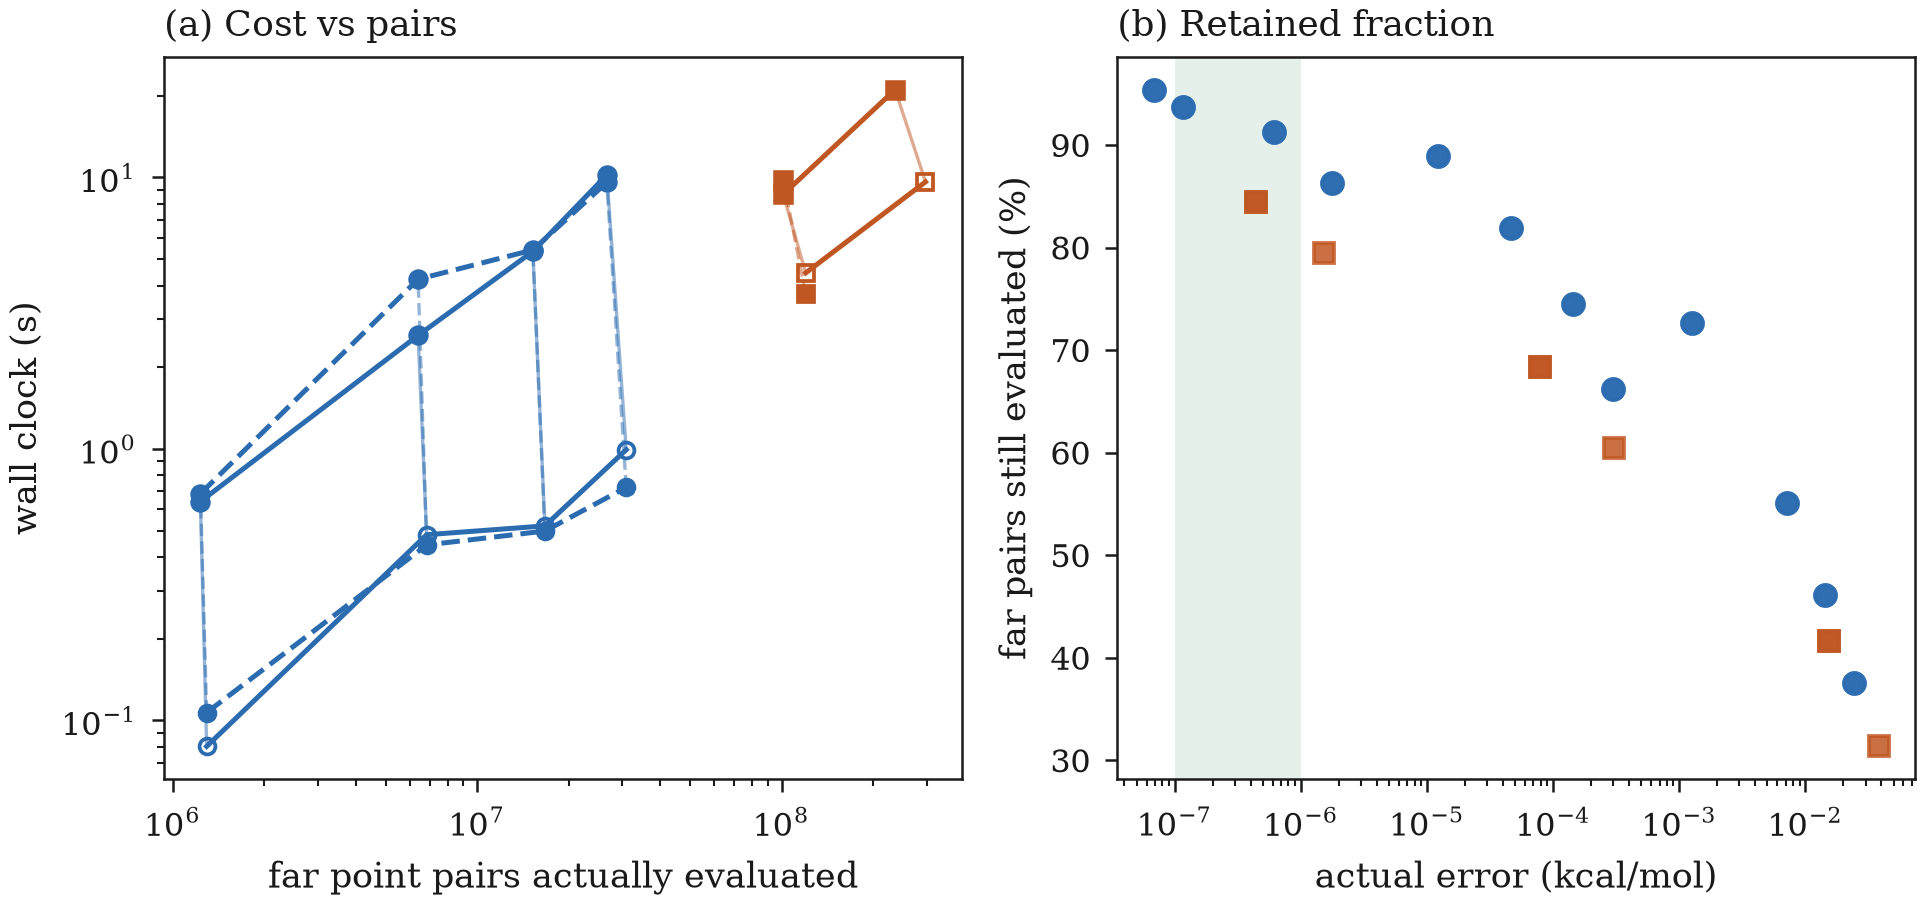
\includegraphics[width=0.92\textwidth]{figs/fig3_screening_cost.png}
\caption{\textbf{Figure 1.} Every run that passes the contention gate is drawn: 6 from \texttt{evidence/scaling/step\_j.json} and 5 from \texttt{evidence/scaling/step\_j\_rerun\_20260930.json}, because the claim above is about all 33 screened/exact pairs, and a figure that dropped the second window would quietly drop a number that counts against us. Panel (a) draws those 11 runs, two markers and one connector per run: each connector joins a system's exact run to its own $\tau$ = 1e-12 screened run at the same grid level, so a connector that rises while moving left reads "less work, more time" for that system. Hollow markers on solid lines are the archived window, filled markers on dashed lines the rerun. Panel (b) draws 33 points, one per run and tolerance. The green band in panel (b) is drawn between 1e-7 and 1e-6 kcal/mol; the accuracy this decomposition is used at is |$\Delta$E| $\leq$ 1e-6, so the two 3-atom points, at 6.8e-8, sit to the left of the band while still meeting that target. 8 of the 33 timed pairs meet it, and inside that set the screened path is still evaluating 84.4-95.4\% of the far point pairs. Drawn by \texttt{nlcsplit/figures.py} from the two cited artefacts; panel (a) plots a window's level group even when the group holds a single run, which matters here because the rerun window has exactly one level-1 row.}
\label{fig:1}
\end{figure}

\section{7. What would have to be true for this to pay}

Stated as conditions we did not meet, so the reader can check them against their own system before implementing anything:

1. \textbf{The bound must clear the target at coarse granularity.} At atom-pair granularity the    \emph{smallest} block-pair bound we found in a real dimer is 197.96 Ha against a quantity of    $-$8.34e-4 Ha, with \texttt{n\_pairs\_bound\_below\_value = 0} and \texttt{dropped\_pairs = []}    [\texttt{evidence/fastpair\_ab/fastpair\_ab\_compare.json}, \texttt{ide\_full} and \texttt{ide\_tau1em8} rows of    the built-geometry dimer]. The comparison sidecar    [\texttt{evidence/fastpair\_ab/fastpair\_ide\_validation.json}] carries the same 197.96 Ha as    \texttt{min\_block\_bound\_ha} and \texttt{n\_dropped\_screen = 0}, but neither of the two fields just named,    and its copy of the bound differs in the last digits (\ldots{}49376 against \ldots{}48444 Ha). No    traversal can fix a bound that is loose by 2.4e5$\times$; it can only descend, and descent is    what costs. 2. \textbf{Most pairs must be droppable at the target accuracy.} At the coarsest $\tau$ in the sweep    that meets \texttt{|dE| $\leq$ 1e-6} kcal/mol, the screened path still evaluates 84.4-95.4\% of the    far point pairs (droppable share 4.6-15.6\%) --- and for two of the six systems (12 atoms at    level 0, 9 atoms at level 1) no $\tau$ in the sweep meets the target at all, so their    admissible $\tau$ is finer and the share smaller. 3. \textbf{The per-pair decision must be cheaper than the arithmetic it avoids.} Measured false:    the tree is cheaper than the large gemm on \textbf{0 of 15} root pairs, and the near field is    100\% of the cross point pairs (all 15 root box gaps are exactly 0.0000 \AA{}, printed by the    root-separation check in \texttt{evidence/fastpair\_ab/20260929T105823Z\_pytest\_fastpair\_L2\_L4.out}). 4. \textbf{The system must have a far field at all.} Our ladder is a chain at fixed density;    compact dimers (S22) have no inter-block region that is both distant and negligible.    A 300-atom protein-ligand complex with genuinely separated fragments is outside what we    measured, and we make no claim about it.

Condition 1 is structural for VV10 as implemented in PySCF: the kernel's \texttt{g} is \texttt{w0(r\_j) R$^{2}$ + $\kappa$(r\_i)}, and \texttt{w0} contains \texttt{(4$\pi$/3)$\rho$} under a square root, so a \emph{low-density} grid point carries a small \texttt{w0} and a huge bound. The tail points that inflate the boxes are the same points that fail to make the bound decay. That coupling is why the atom-block bound is loose, why refinement is the only mechanism that fires, and why refinement does not pay.
\bibliographystyle{unsrtnat}
\bibliography{references-p2}
\end{document}
